\documentclass[12pt,t]{beamer}
\usepackage{graphicx}
\beamerdefaultoverlayspecification{<+->}
\setbeameroption{hide notes}
\setbeamertemplate{note page}[plain]
\usepackage{listings}
\usepackage{datetime}
\usepackage{url}

\usepackage{amsmath}
\usepackage{amsfonts}
\usepackage{amssymb}
\usepackage{mathptmx}
\usepackage{dsfont}
\usepackage{psfrag}
\usepackage{epsfig}
\usepackage{float}
\usepackage{breqn}
\usepackage{bbm}

%Bibliography
\usepackage{natbib}
\bibpunct{(}{)}{,}{a}{}{;}
\usepackage{bibentry}
\nobibliography*

% header.tex: boring LaTeX/Beamer details + macros

% get rid of junk
\usetheme{default}
\beamertemplatenavigationsymbolsempty
\hypersetup{pdfpagemode=UseNone} % don't show bookmarks on initial view


% font
\usepackage{fontspec}
\setsansfont
  [ ExternalLocation = fonts/ ,
    UprightFont = *-regular ,
    BoldFont = *-bold ,
    ItalicFont = *-italic ,
    BoldItalicFont = *-bolditalic ]{texgyreheros}
\setbeamerfont{note page}{family*=pplx,size=\footnotesize} % Palatino for notes
% "TeX Gyre Heros can be used as a replacement for Helvetica"
% I've placed them in fonts/; alternatively you can install them
% permanently on your system as follows:
%     Download http://www.gust.org.pl/projects/e-foundry/tex-gyre/heros/qhv2.004otf.zip
%     In Unix, unzip it into ~/.fonts
%     In Mac, unzip it, double-click the .otf files, and install using "FontBook"

% named colors
\definecolor{offwhite}{RGB}{255,250,240}
\definecolor{gray}{RGB}{155,155,155}

\ifx\notescolors\undefined % slides
  \definecolor{foreground}{RGB}{255,255,255}
  \definecolor{background}{RGB}{24,24,24}
  \definecolor{title}{RGB}{107,174,214}
  \definecolor{subtitle}{RGB}{102,255,204}
  \definecolor{hilit}{RGB}{102,255,204}
  \definecolor{vhilit}{RGB}{255,111,207}
  \definecolor{lolit}{RGB}{155,155,155}
\else % notes
  \definecolor{background}{RGB}{255,255,255}
  \definecolor{foreground}{RGB}{24,24,24}
  \definecolor{title}{RGB}{27,94,134}
  \definecolor{subtitle}{RGB}{22,175,124}
  \definecolor{hilit}{RGB}{122,0,128}
  \definecolor{vhilit}{RGB}{255,0,128}
  \definecolor{lolit}{RGB}{95,95,95}
\fi
\definecolor{nhilit}{RGB}{128,0,128}  % hilit color in notes
\definecolor{nvhilit}{RGB}{255,0,128} % vhilit for notes

\newcommand{\hilit}{\color{hilit}}
\newcommand{\vhilit}{\color{vhilit}}
\newcommand{\nhilit}{\color{nhilit}}
\newcommand{\nvhilit}{\color{nvhilit}}
\newcommand{\lolit}{\color{lolit}}

% use those colors
\setbeamercolor{titlelike}{fg=title}
\setbeamercolor{subtitle}{fg=subtitle}
\setbeamercolor{institute}{fg=lolit}
\setbeamercolor{normal text}{fg=foreground,bg=background}
\setbeamercolor{item}{fg=foreground} % color of bullets
\setbeamercolor{subitem}{fg=lolit}
\setbeamercolor{itemize/enumerate subbody}{fg=lolit}
\setbeamertemplate{itemize subitem}{{\textendash}}
\setbeamerfont{itemize/enumerate subbody}{size=\footnotesize}
\setbeamerfont{itemize/enumerate subitem}{size=\footnotesize}

% page number
\setbeamertemplate{footline}{%
    \raisebox{5pt}{\makebox[\paperwidth]{\hfill\makebox[20pt]{\lolit
          \scriptsize\insertframenumber}}}\hspace*{5pt}}

% add a bit of space at the top of the notes page
\addtobeamertemplate{note page}{\setlength{\parskip}{12pt}}

% default link color
\hypersetup{colorlinks, urlcolor={hilit}}

\ifx\notescolors\undefined % slides
  % set up listing environment
  \lstset{language=bash,
          basicstyle=\ttfamily\scriptsize,
          frame=single,
          commentstyle=,
          backgroundcolor=\color{darkgray},
          showspaces=false,
          showstringspaces=false
          }
\else % notes
  \lstset{language=bash,
          basicstyle=\ttfamily\scriptsize,
          frame=single,
          commentstyle=,
          backgroundcolor=\color{offwhite},
          showspaces=false,
          showstringspaces=false
          }
\fi

% a few macros
\newcommand{\bi}{\begin{itemize}}
\newcommand{\bbi}{\vspace{24pt} \begin{itemize} \itemsep8pt}
\newcommand{\ei}{\end{itemize}}
\newcommand{\ig}{\includegraphics}
\newcommand{\subt}[1]{{\footnotesize \color{subtitle} {#1}}}
\newcommand{\ttsm}{\tt \small}
\newcommand{\ttfn}{\tt \footnotesize}
\newcommand{\figh}[2]{\centerline{\includegraphics[height=#2\textheight]{#1}}}
\newcommand{\figw}[2]{\centerline{\includegraphics[width=#2\textwidth]{#1}}}


%%%%%%%%%%%%%%%%%%%%%%%%%%%%%%%%%%%%%%%%%%%%%%%%%%%%%%%%%%%%%%%%%%%%%%
% end of header
%%%%%%%%%%%%%%%%%%%%%%%%%%%%%%%%%%%%%%%%%%%%%%%%%%%%%%%%%%%%%%%%%%%%%%

% title info
\title{Empirical Bayes Moderation of Asymptotically Linear Parameters}
\author{\href{http://nimahejazi.org}{Nima Hejazi}}
\institute{Division of Biostatistics \\
           University of California, Berkeley \\
           \href{https://www.stat.berkeley.edu/~nhejazi}
             {\tt \scriptsize \color{foreground} stat.berkeley.edu/\textasciitilde{}nhejazi}
          }
\date{
  \href{http://nimahejazi.org}
      {\tt \scriptsize \color{foreground} nimahejazi.org}
  \\[-4pt]
  \href{https://twitter.com/nshejazi}
      {\tt \scriptsize \color{foreground} twitter/@nshejazi}
  \\[-4pt]
  \href{https://github.com/nhejazi}
      {\tt \scriptsize \color{foreground} github/nhejazi}
}


\begin{document}

% title slide
{
\setbeamertemplate{footline}{} % no page number here
\frame{
  \titlepage

  \vspace{-2em}

  \centerline{\href{https://goo.gl/6ou8YR}{\tt \scriptsize \underline{slides}: goo.gl/6ou8YR}}

  \vfill \hfill 
\includegraphics[height=6mm]{Figs/cc-zero.png} \vspace*{-0.75cm}

  \note{These are slides for a talk given most recently at the Division of
    Biostatistics seminar series, at the University of California, Berkeley on
    20 March 2017.

    Source: {\tt https://github.com/nhejazi/talk\_biotmle} \\
    Slides: {\tt https://goo.gl/r3zsu6} \\
    With notes: {\tt https://goo.gl/6ou8YR}
}
}
}



\begin{frame}[c]{Preview}
\only<1>{\addtocounter{framenumber}{-1}}
\begin{center}
\begin{enumerate}
  \itemsep12pt
  \item Linear models are the standard approach for analyzing microarray and
    next-generation sequencing data (e.g., R package ``limma'').
  \item Moderated statistics help reduce false positives by using an empirical
    Bayes method to perform standard deviation shrinkage for test statistics.
  \item \textit{Beyond linear models:} we can assess evidence using parameters
    that are more scientifically interesting (e.g., ATE) by way of TMLE.
  \item The approach of moderated statistics easily extends to the case of
    asymptotically linear parameters.
\end{enumerate}
\end{center}


\note{We'll go over this summary again at the end of the talk. Hopefully, it
      will all make more sense then.
}
\end{frame}



\begin{frame}[c]{Motivation: Let's meet the data}
\begin{center}
\begin{itemize}
  \itemsep12pt
  \item Observational study of the impact of occupational exposure (to benzene),
    with data collected on $125$ subjects and roughly $22,000$ biomarkers.
  \item Biomarkers of interest are in the form of \textbf{miRNA}, assessed
    using the \textit{Illumina Human Ref-8 BeadChips} platform.
  \item Occupational exposure to benzene reported as discrete values of
    interest (to epidemiologists): none, $<1$ppm, $>5$ppm.
  \item Background (phenotype-level) information available on each subject,
    including age, sex, smoking status.
\end{itemize}
\end{center}


\note{This is not an atypical data set by modern standards in epidemiology,
      certainly not the standard for molecular biology. That is, sample sizes
      are usually much smaller in experiments examining biological processes.
}
\end{frame}



\begin{frame}[c]{Data analysis? Linear models!}
\begin{center}
\begin{itemize}
  \itemsep12pt
  \item For each biomarker ($b = 1, \dots, B$), fit a linear model:
    \[
    \mathbb{E}[y_b] = X \beta_b
    \]
  \item Generally, we have a particular model coefficent in which we are
    interested (e.g., effect of benzene on biomarker expression).
  \item Controlling for baseline covariates, batch effects, and potential
    confounders happens by adding terms to the linear model.
  \item Test the coefficent of interest using a standard t-test:
    \[
      t_{b} = \frac{\hat{\beta}_{b} - \beta_{b, H_0}}{s^2_b}
    \]
\end{itemize}
\end{center}


\note{There's nothing particularly wrong with this approach. It's exactly what
      we would come up with after a first-year statistics course. In practice,
      there are many issues: (1) we are forced to specify a functional form, the
      linear model; (2) we end up with unstable variance estimates that sharply
      increase the number of false positives detected, even after multiple
      testing corrections.
}
\end{frame}



\begin{frame}[c]{LIMMA: Linear Models for Microarray Data}

\begin{center}
\begin{itemize}
  \itemsep12pt
  \item When the sample size is small, $s^2_b$ may be so small that small
    differences ($\hat{\beta}_{b} - \beta_{b, H_0}$) lead to large $t_{b}$.
  \item Uncertainty in the variance is an acute problem when the sample size is
    small.
  \item This results in false positives. Smyth proposes we get around this by an
    empirical Bayes shrinkage of the $s^2_b$.
  \item Test the coefficent of interest with a \textbf{moderated} t-test:
    \[
      \tilde{t}_{b} = \frac{\hat{\beta}_{b} - \beta_{b, H_0}}{\tilde{s}^2_b},
      \,
      \tilde{s}^2_b = \frac{s^2_bd_b + s^2_0d_0}{d_b + d_0}
    \]
  \item Eliminates large t-statistics merely from very small $s_b$.
\end{itemize}
\end{center}

\note{The substantive contribution here is the use of an empirical Bayes method
      to shrink the standard deviation across all of the biomarkers such that we
      obtain a larger (but accurate) estimate that reduces the number of test
      statistics that are marked as significant by low $s^2_b$ estimates alone.
}
\end{frame}



\begin{frame}[c]{Beyond linear models}

\begin{center}
\begin{itemize}
  \itemsep12pt
  \item It's not always desirable to specify a functional form: perhaps we can
    do better than linear models?
  \item Such models are a matter of convenience and not honest scientific
    practice: does $\hat{\beta}_{b}$ really answer our questions?
  \item We can do better by using parameters motivated by causal models (n.b.,
    these will reduce to ``variable importance measures'' in our case).
  \item As long as the parameters we seek to estimate have asymptotically linear
    estimators, we can readily apply the approach of moderated statistics.
\end{itemize}
\end{center}

\note{Linear models are convenient for communicating results --- that is, all
      scientists are trained to understand them. This means they provide a basic
      way of easily communicating between statisticians and collaborators. That
      said, doesn't it seem a bit odd to use such elementary models to analyze
      complex biological sequencing data? We're using old statistical technology
      to analyze classes of data that have only recently become available.
}
\end{frame}



\begin{frame}[c]{Target parameters for complex questions}

\begin{center}
\begin{itemize}
  \itemsep12pt
  \item Rather than being satisfied with $\hat{\beta}_{b}$ as an answer to our
    questions, let's consider a simple target parameter: the average treatment
    effect (ATE):
    \[
      \Psi_b(P_0) = \mathbb{E}_{W,0}[\mathbb{E}_0[Y_b \mid A = a_{high}, W] -
      \mathbb{E}_0[Y_b \mid A = a_{low}, W]]
    \]
  \item No need to specify a functional form or assume that we know the true
    data-generating distribution $P_0$.
  \item Parameters like this can be estimated using \textit{targeted minimum
    loss-based estimation} (TMLE).
  \item \textbf{Asymptotic linearity:}
    \[
      \sqrt{n}(\Psi_b(P_n^*) - \Psi_b(P_0)) = \frac{1}{\sqrt{n}}
      \sum_{i = 1}^{n} IC(O_i) + o_P(1)
    \]
\end{itemize}
\end{center}

\note{By allowing scientific questions to inform the parameters that we choose
      to estimate, we can do a better job of actually answering the questions of
      interest to our collaborators. Further, we abandon the need to specify the
      functional relationship between our outcome and covariates; moreover, we
      can now make use of advances in machine learning.
}
\end{frame}



\begin{frame}[c]{Targeted Minimum Loss-Based Estimation}

\begin{center}
\begin{itemize}
  \itemsep12pt
  \item TMLE produces a well-defined, unbiased, efficient substitution estimator
    of target parameters of a data-generating distribution.
  \item Iterative procedure (though there is a one-step now) that updates an
    initial estimate of the relevant part ($Q_0$) of the data generating
    distribution ($P_0$).
  \item Like corresponding A-IPTW estimators, removes asymptotic residual bias
    of initial estimator for the target parameter. If it uses a consistent
    estimator of $g_0$ (nuisance parameter), it is \textit{doubly robust}.
  \item We can estimate the target parameter:
    \[
      \Psi_b(P_n^*) = \frac{1}{n}\sum_{i=1}^{n}[Q_n^{(b,1)}(A_i = a_h, W_i) -
      Q_n^{(b,1)}(A_i = a_l, W_i)]
    \]
\end{itemize}
\end{center}

\note{Natural use of machine learning methods for the estimation of both $Q_0$
      and $g_0$. Focuses effort to achieve minimal bias and asymptotic
      semiparametric efficiency bound for the variance, but still get inference
      (with some assumptions).
}
\end{frame}




\begin{frame}[c]{Inference with influence curves}

\begin{center}
\begin{itemize}
  \itemsep12pt
  \item The influence curve for the estimator is:
  \begin{dmath}
    IC_{b,n}(O_i) = \left (\frac{\mathbbm{1}(A_i = a_{h})}{g_n(a_{h} \mid W_i)}
    - \frac{\mathbbm{1}(A_i = a_{l})}{g_n (a_{l} \mid W_i)} \right) \cdot
    (Y_{b,i} - \bar{Q}^{(b,1)}_n(A_i, W_i)) +
    \bar{Q}^{(b,1)}_n(a_{h}, W_i) - \bar{Q}^{(b,1)}_n(a_{l}, W_i) -
    \Psi_{b}(P_n^*)
  \end{dmath}
  \item Sample variance of the estimated influence curve:
    \[
      \textstyle s^2(IC_n) = \frac{1}{n}\sum_{i=1}^n\left(IC_n(O_i) \right)^2
    \]
  \item Use sample variance to estimate the standard error:
    \[
      se_n = \sqrt{\frac{s^2(IC_n)}{n}}
    \]
  \item Use this for inference --- that is, to derive uncertainty measures
    (p-values, confidence intervals).
\end{itemize}
\end{center}

\note{Using the influence curve representation, we can obtain all of the
  standard objects of statistical interest, but for more interesting parameters.
}
\end{frame}



\begin{frame}[c]{Moderated statistics for target parameters}

\begin{center}
\begin{itemize}
  \itemsep12pt
  \item One can define a standard t-test statistic for an estimator of an
    asymptotically linear parameter (over $b = 1, \dots, B$) as:
    \[
      t_b = \frac{\sqrt{n}(\Psi_b(P_n^*) - \Psi_0)}{s_b(IC_{b,n})}
    \]
  \item This naturally extends to the moderated t-statistic of Smyth:
    \[
      \tilde{t}_b = \frac{\sqrt{n}(\Psi_b(P_n^*) - \Psi_0)}{\tilde{s}_b^2}
    \]
    where the posterior estimate of the variance of the influence curve is
    \[
      \tilde{s}^2_b = \frac{s^2_b(IC_{b,n})d_b + s^2_0d_0}{d_b + d_0}
    \]
\end{itemize}
\end{center}

\note{
  \begin{itemize}
    \item Consider this is repeated for $b = 1, \ldots, B$  different
      biomarkers, so that one has, for each $b$:
      $$\Psi_b(Q_{b,n}^{*}), S_b^2(IC_{b,n}),$$
      estimate of variable importance and standard error for all $B$.
    \item Propose an existing joint-inferential procedure that can add some
      finite-sample robustness to an estimator that can be highly variable.
   \end{itemize}
}
\end{frame}



\begin{frame}[c]{An influence curve transform}

\begin{center}
\begin{itemize}
  \itemsep12pt
  \item Need the estimate for each biomarker ($b$) and the IC for every
    observation for that biomarker, repeating for all $b = 1, \dots, B$.
  \item Essentially, transform original data matrix such that new entries are:
    \[
      Y^*_{b,i} = IC_{b,n}(O_i; P_n) + \Psi_b(P_n^*)
     \]
 \item Since $\mathbb{E}[IC_{b,n}] = 0$ across the columns (units) for each $b$,
   the average will be the original estimate $\Psi_b(P_n^*)$.
  \item For simplicity, let's assume the null value is $\Psi_0 = 0$ for all $b$.
    Then, applying the moderated t-test to $Y^*_{b,i}$ will generate corrected,
    conservative test statistics $\tilde{t}_b$.
\end{itemize}
\end{center}

\note{Just like the one-sample problem for estimation of parameter with
    associated standard error from the influence curve.}
\end{frame}



\begin{frame}[c]{Why moderated statistics in this context?}

\begin{center}
\begin{itemize}
  \item Often times, such data analyses are based on relatively small samples.
  \item To get a data-adaptive estimate, with standard implementation of these
    estimates, standard errors can be non-robust.
\item Practically, ``significant'' estimates of variable importance measures may
  be driven by poorly and underestimated $s^2_b(IC_{b,n})$.
\item Moderated statistics shrink these $s^2_b(IC_{b,n})$ (making them bigger),
  thus taking biomarkers with small parameter estimates but very small
  $s^2_b(IC_{b,n})$ out of statistical significance.
\end{itemize}
\end{center}

\note{Essentially, we have the same concerns about using variable importance
  measures that we did about using the standard t-test --- that is, non-robut
  estimates of the standard error of the estimator of the target parameter can
  cause erroneous identification of biomarkers (false positives). To reduce
  this, we can apply the same machinery that we did in the case of the standard
  t-test for our naive linear modeling approach.
}
\end{frame}



\begin{frame}[c]{Software implementation: ``R/biotmle''}

\begin{center}
\begin{itemize}
  \itemsep12pt
  \item An R package that ``facilitates biomarker discovery by generalizing the
    moderated t-statistic of Smyth for use with asymptotically linear
    parameters.''
  \item Check it out on GitHub: \href{https://github.com/nhejazi/biotmle}
    {nhejazi/biotmle} \\[1em]
    \includegraphics<2->[width=.92\textwidth]{Figs/biotmle.png}
\end{itemize}
\end{center}

\note{Use it. File an issue. Help make it better!
}
\end{frame}



\begin{frame}[c]{Data analysis with ``R/biotmle''}

\begin{center}
\begin{itemize}
  \itemsep12pt
  \item Observational study of the impact of occupational exposure (to benzene),
    with data collected on $125$ subjects and roughly $22,000$ biomarkers.
  \item Baseline covariates $W$: age, sex, smoking status; all were discretized.
  \item Treatment $A$ is degree of Benzene exposure: none, $<1$ppm, and $>5$ppm.
  \item Outcome $Y$ is miRNA expression, median normalized.
  \item Estimate the parameter:
    \[
      \Psi_b(P_n^*) = \mathbb{E}[\mathbb{E}[Y_b \mid A = \text{max}(A), W] -
      \mathbb{E}[Y_b \mid A = \text{min}(A), W]]
    \]
  \item Apply moderated t-test as previously discussed.
\end{itemize}
\end{center}

\note{We are really just walking through the mechanistic procedure we outline,
      applying to the data set that served as our motivating example.
}
\end{frame}



\begin{frame}[c]{Analysis results I: Uncorrected tests}

\begin{center}
  \includegraphics[scale=0.47]{Figs/limma_rawp.pdf}
\end{center}

\note{This is promising --- we're not seeing too many biomarkers identified as
      ``significant.'' But, we do have to correct for those $22,000$ tests that
      we just performed.
}
\end{frame}



\begin{frame}[c]{Analysis results II: Corrected tests}

\begin{center}
  \includegraphics[scale=0.47]{Figs/limma_adjp.pdf}
\end{center}

\note{After application of the Benjamini-Hochberg procedure for controlling the
      False Discovery Rate (FDR).
}
\end{frame}



\begin{frame}[c]{Analysis results III: Heatmap of IC estimates}

\begin{center}
  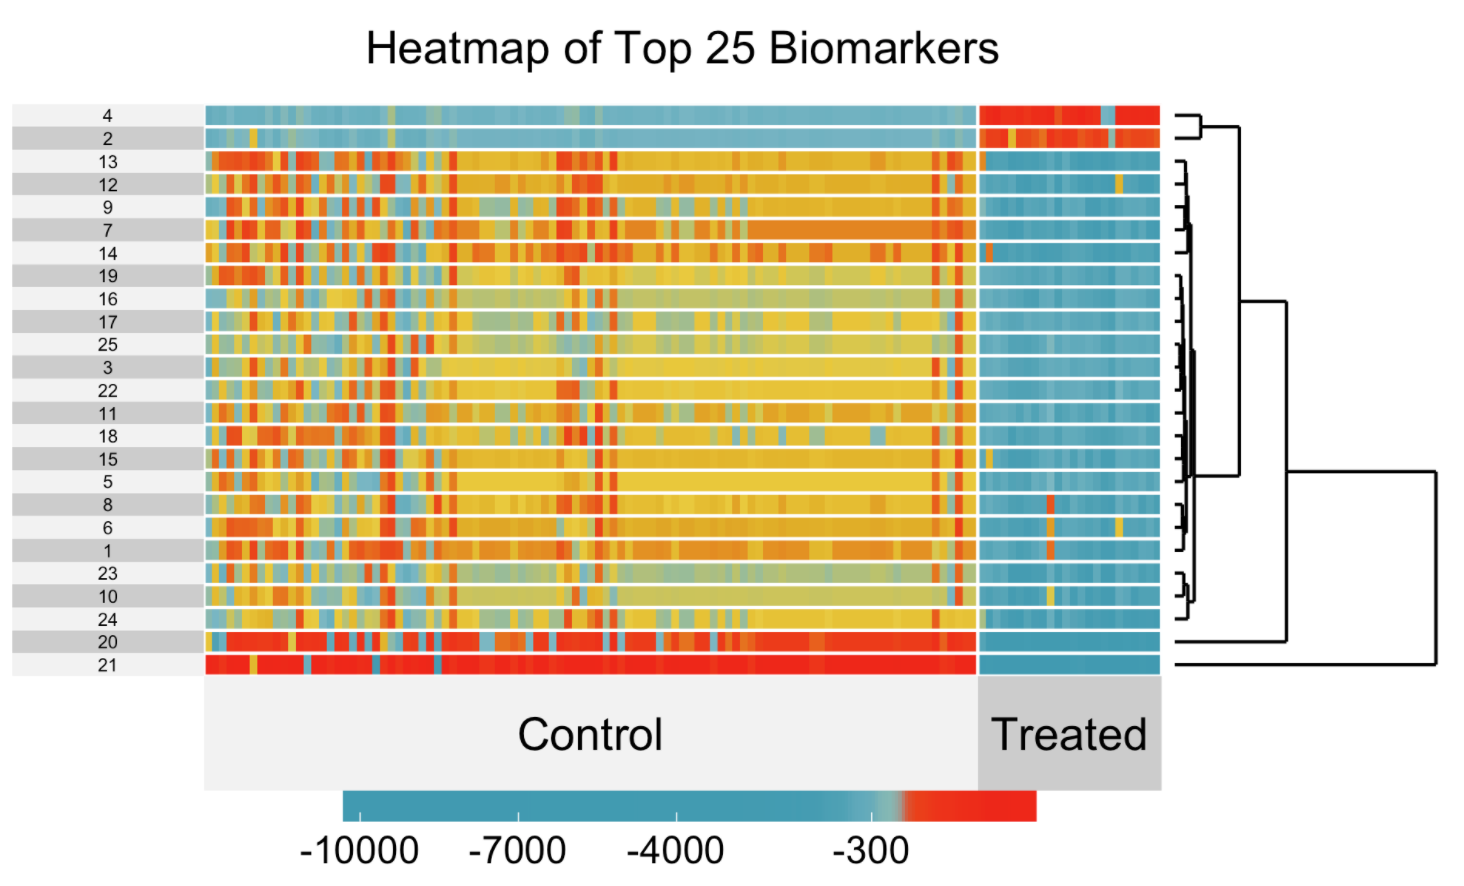
\includegraphics[scale=0.45]{Figs/superheatmap.png}
\end{center}

\note{We can use our influence curve transform to identify biomarkers that are
      top contributers to the target parameter of interest --- the ATE in this
      case.
}
\end{frame}



\begin{frame}[c]{Review}
\begin{center}
\begin{enumerate}
  \itemsep12pt
  \item Linear models are the standard approach for analyzing microarray and
    next-generation sequencing data (e.g., R package ``limma'').
  \item Moderated statistics help reduce false positives by using an empirical
    Bayes method to perform standard deviation shrinkage for test statistics.
  \item \textit{Beyond linear models:} we can assess evidence using parameters
    that are more scientifically interesting (e.g., ATE) by way of TMLE.
  \item The approach of moderated statistics easily extends to the case of
    asymptotically linear parameters.
\end{enumerate}
\end{center}


\note{It's always good to include a summary.}
\end{frame}



\begin{frame}{Acknowledgments}
\vspace{18pt}
\begin{tabular}{@{}l@{\hspace{1.5cm}}l@{}}
Alan Hubbard & \footnotesize \lolit University of California, Berkeley \\
\\[0.5ex]
Mark van der Laan & \footnotesize \lolit University of California, Berkeley \\

%\\[2ex]

%Collaborator, the first & \footnotesize \lolit University or Institution 2 \\
%Collaborator, the second & \footnotesize \lolit University or Institution 2 \\
\end{tabular}

\vspace{10mm}

%NIH - funding source ?

\note{This was all made possible by generous advising and collaboration.}
\end{frame}



\begin{frame}[c]{}

\Large
Slides: \href{https://goo.gl/6ou8YR}{goo.gl/6ou8YR} \quad

\includegraphics[height=5mm]{Figs/cc-zero.png}

\vspace{10mm}

\href{https://www.stat.berkeley.edu/~nhejazi}{\tt stat.berkeley.edu/\textasciitilde{}nhejazi}

\vspace{10mm}

\href{http://nimahejazi.org}{\tt nimahejazi.org}

\vspace{10mm}

\href{https://twitter.com/nshejazi}{\tt twitter/@nshejazi}

\vspace{10mm}

\href{https://github.com/nhejazi}{\tt github/nhejazi}


\note{Here's where you can find me, as well as the slides for this talk.}
\end{frame}



\end{document}
